
\documentclass{beamer}
 
\usepackage[utf8]{inputenc}
\usepackage{tikz}
\newcommand\Algorithm{%
  \textbf{Algorithm:}\\%
}
\newcommand\Notation{%
  \textbf{Notation}\\%
}
 
\usetheme{Szeged}
\usecolortheme{seahorse}
 
%Information to be included in the title page:
\title[Matroids] %optional
{Matroids for solving Optimisation Problems}
 
\subtitle{The Greedy algorithm as a solution}

\author{emcd123}
\institute{NUI Galway}
\date{2018}
 
\begin{document}
 
\frame{\titlepage}
 
\begin{frame}
\frametitle{The Problem}
\begin{minipage}{.2\textwidth}
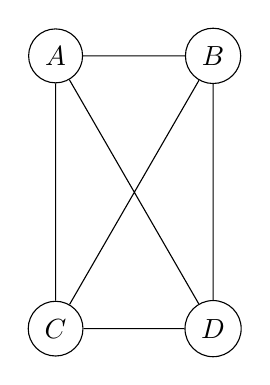
\begin{tikzpicture}
    \tikzstyle{every node}=[draw,shape=circle];
    \node (A) at (1*60:2) {$B$};
    \node (B) at (2*60:2) {$A$};
    \node (D) at (4*60:2) {$C$};
    \node (E) at (5*60:2) {$D$};
    \draw (B) -- (D)
          (B) -- (A)
          (A) -- (E)
          (B) -- (E)
          (A) -- (D)
          (D) -- (E);
\end{tikzpicture}
\end{minipage}
\hspace{2.5cm} \begin{minipage}{.5\textwidth}
Let $G$ be $K_4$ as seen here, where the vertices correspond to towns to be linked by railway network, and the weight on each edge is the cost of providing a link between the towns correspnding to the respective vertices. In this case, the minimum weight of a spanning tree in $G$ corrsponds to the minimum cost of providing a railway that will link all $n$ towns.
\end{minipage}
\end{frame}

\begin{frame}
\frametitle{Greedy Algorithm}
Kruskal's algorithm is a greedy algorithm that finds a minimum spanning tree for a connected weighted Graph.

\vspace{4mm}

\Algorithm
$1)$ Create a graph $F$(a set of trees) where each vertex of G is a separate tree.\\
$2)$ Create a set $S$ conatining all the edges of the graph.\\
$3)$ While $S$ is non-empty and $F$ is not yet spanning\\
\hspace{5mm} $3(a)$ Remove an edge with minimum weight from S.\\
\hspace{5mm} $3(b)$ If the removed edge connects two different trees then add \\
\hspace{5mm} it to the forest $F$, combining two trees into a single tree.\\
	


\end{frame}

\begin{frame}
\frametitle{Why Greedy works?}

\begin{lemma}
If $(E,\mathcal{I})$ is a matroid $M,$ then $B_G$ is a solution to the optimization problem.
\end{lemma}


Where $B_G$ is a spanning tree created through the greedy algorithm.


\vspace{5mm}

But what is a matroid?

\end{frame}


\begin{frame}
\frametitle{Independence Systems and Matroids}
\begin{definition}
An \textit{independence system} is a pair $(E,\mathcal{S}),$ where $E$ is a set and $\mathcal{S}$ is a non-empty subset of the power set of $E$, closed under inclusion. The elements of $\mathcal{S}$ are called the \textit{independent sets}.
\end{definition}
\begin{definition}
A matroid is a pair $(E,\mathcal{I})$ with finite ground set E and $\mathcal{I}$ being a collection of independent subsets of E satisfying the following conditions

\vspace{2mm}

 \noindent (I1): The empty set is always independent\\
 \noindent (I2): Every subset of an independent set is independent\\
 \noindent (I3): If $ A $ and $ B $ are two independent sets in $\mathcal{I}$ and $|A|=|B|+1$, then there exists $ x \in A \setminus B $ such that $ B \cup \{ x \} $ is in $\mathcal{I}$
\end{definition}

\end{frame}

\begin{frame}
\frametitle{Bases of a Matroid}
 
\begin{definition}
A base is a maximally independent subset of $\mathcal{I}.$\\
\noindent All the maximally independent sets have the same cardinality, this is the \textit{rank} of the matroid.
\end{definition}
\begin{definition}
  Let $\mathcal{B}$ be a set of subsets of a finite set E. Then $\mathcal{B}$ is the collection of bases of a matroid on E if and only if $\mathcal{B}$ satisfies the following conditions:\\
 (B1) $\mathcal{B}$ is non-empty.\\
 (B2) If $B_1$ and $B_2$ are members of $\mathcal{B}$ and $x \in B_1 \setminus B_2$, then there is an element $y$ of $B_1 \setminus B_2$ such that $(B_1 \setminus \{x\}) \cup \{y\} \in \mathcal{B}$.
 \end{definition}
\end{frame}

\begin{frame}
\frametitle{Spanning trees are Bases}
\begin{definition}
A spanning tree $T$ of an undirected graph $G$ is a subgraph that is a \textit{tree} which includes all of the vertices of $G$, with minimum possible number of edges.\\
Also $T$ does not contain any cycles, but adding any further edge yields a cycle, so $T$ is maximal in $G$.\\
\end{definition}
\begin{lemma}
Any acyclic graph on $n$ vertices has at most $n-1$ edges. And a spanning tree has exactly $n-1$ edges.
\end{lemma}
From this we can see, that if $\mathcal{B}$ is the collection of maximally elements of $\mathcal{I}$, then in $G$, $\mathcal{B}$ is the set of spanning trees of the graph.
\end{frame}

\begin{frame}
\frametitle{Weight Function}
The optimization problem associated with $(E,\mathcal{S)}$ is the following: for a given weight function $\omega : E \rightarrow \mathbb{R^{+}}$, we want to find an independent set $A$ whose weight,
\begin{equation}
\omega(A) := \sum_{e \in A} \omega (e)
\end{equation}
is maximal.
\end{frame}

\begin{frame}
\frametitle{Greedy Weight funtion}
\begin{lemma}
If $(E,\mathcal{I})$ is a matroid $M,$ then $B_G$ is a solution to the optimization problem.
\end{lemma}
\begin{proof}
If $r(M) = r,$ then $B_G = \{e_1,e_2, ..., e_r\}$ is a basis of $M.$ Let $B$ be another basis of $M$, $B = \{f_1, f_2, ..., f_r\}$
where $\omega(f_1) \geq \omega(f_2) \geq ... \geq \omega(f_r).$ This follows from the result of the next additional lemma showing that not only is $B_G$ a maximum weight basis of $M$ ,but is also at least as heavy as the elements of $B$ at each step.\\
\end{proof}
\end{frame}

\begin{frame}
\frametitle{Continued}
\begin{lemma}
if $1 \leq j \leq r,$ then $\omega(e_j) \geq \omega(f_j).$
\end{lemma}
\begin{proof}
Suppose(seeking a contradiction) that $k$ is the least integer for which $\omega(e_k) \leq \omega(f_k).$ Take $I_1 = \{e_1, e_2, ..., e_{k-1}\}$ and $I_1 = \{f_1, f_2, ..., f_{k-1}\}.$ Since $|I_1| = |I_2|+1$ by $(I3)$ implies $I_1 \cup \{f_t\} \in \mathcal{I}$ for some $f_t \in I_2 \setminus I_1.$ But this means that $\omega(f_t) \geq \omega(f_t) > \omega(e_k).$ Hence the Greedy algorithm would have chosen $f_t$ over $e_k$, which gives us our contradiction.
\end{proof}

\end{frame}

\begin{frame}
\frametitle{Wrap Up}
The combination of the previous lemma and our use of the greedy algorithm to find a maximal member $B$ of $\mathcal{I}$ of maximum weight allows us to deduce that Kruskal's algorithm does generate a minimum weight spanning tree of a graph. \\We have seen that greedy algorithm gives us a solution to our optimisation problem as long as we have a matroid.
\end{frame}

\end{document}

